\runningheader{SAT Mathematics}{Drill Set 13}{Page \thepage\ of \numpages}

\begingradingrange{sat-drill-13}
\subsection*{SAT Drill 13}

\question[1]
The given quartic function $54x^4 + 216x^2 + 210$ has factors in the form $(k)(a x^2 + b)(c x^2 + d)$. If $a, b, c, d$, and $k$ are integers, what is the smallest possible value of $ab$?
\begin{solution}
15
\end{solution}

\question[1]
Let
\[
  f(x) = a\left((x+9)^2 - b\right)\left((x+9)^2 - c\right)
\]
where $a, b$, and $c$ are constants. The graph $y = f(x)$ passes through the points $(-14, 15)$ and $(-3, 299)$. What is the value of $f(-4) + f(-15)$?
\begin{solution}
314
\end{solution}

\question[1]
For the function $f$, for each increase in the value of $x$ by $c$, where $c$ is a positive constant, the value of $f(x)$ increases by a factor of $27$. Which of the following equivalent forms of the function $f$ has $\frac{1}{c}$ as a coefficient of $x$?
\begin{choices}
  \choice $f(x) = 48(3)^{\frac{1}{2}x}$
  \CorrectChoice $f(x) = 48\left(3^3\right)^{\frac{1}{6}x}$
  \choice $f(x) = 48(9)^{\frac{1}{4}x}$
  \choice $f(x) = 48\left(27^{\frac{1}{3}x}\right)^{\frac{1}{2}}$
\end{choices}



\newpage




\question[1]
Consider the following system of equations:
\[
  \begin{gathered}
  2x + 3y = 7 \\
  10x + 15y = 35
  \end{gathered}
\]
For each real number $r$, which of the following points lies on the graph of each equation in the $xy$-plane for the given system?
\begin{choices}
  \choice $\left(\frac{r}{5}+7,-\frac{r}{5}+35\right)$
  \CorrectChoice $\left(-\frac{3r}{2}+\frac{7}{2}, r\right)$
  \choice $\left(r, \frac{2r}{3}+\frac{7}{3}\right)$
  \choice $\left(r,-\frac{3r}{2}+\frac{7}{2}\right)$
\end{choices}

\question[1]
Consider the equation:
\[
  (3x + p)\left(5x^2 - 45\right)\left(2x^2 - 16x + 6p\right) = 0
\]
In the given equation, $p$ is a positive constant. The sum of the solutions to the equation is $\frac{20}{3}$. What is the value of $p$?
\begin{solution}
4
\end{solution}

\question[1]
What is the value of $k$ if the given equation only has one solution?
\[
  \frac{1}{4}|x-4|-30=2k
\]
\begin{solution}
-15
\end{solution}


\newpage




\question[1]
Consider the exponential function:
\[
  f(x)=a^x-b
\]
The exponential function given above passes through points $(c, 8)$ and $(2c, 350)$. If $c$ is a positive constant, what is a possible value of $b$?
\begin{solution}
11
\end{solution}

\question[1]
Consider the equation:
\[
  \frac{1}{k}-\frac{x}{63}=\frac{5}{kx}
\]
In the given equation, $k$ is an integer constant. If the equation has more than one solution, what is the greatest possible value of $k$?
\begin{solution}
3
\end{solution}

\question[1]
Consider the equation:
\[
  4x^2+4y^2+bx+by=32
\]
The given equation where $b$ is a positive constant, defines a circle in the $xy$-plane. The radius of the circle is $\sqrt{106}$. What is the value of $b$?
\begin{solution}
56
\end{solution}



\newpage




\question[1]
For two acute angles, $\angle A$ and $\angle B$, $\cos A=\sin B$. The measures, in degrees, of $\angle A$ and $\angle B$ are $13x+10$ and $48+3x$, respectively. What is the value of $x$?
\begin{solution}
2
\end{solution}

\question[1]
Consider the equation:
\[
  \frac{14x+35}{4}-\frac{b}{12}=a(x-7)
\]
In the given equation, $a$ and $b$ are constants. If the equation has infinitely many solutions, what is the value of $b$?
\begin{solution}
399
\end{solution}

\question[1]
The perimeter of an equilateral triangle is 954 inches. The three vertices of the triangle lie on a circle. The radius of the circle is $k\sqrt{3}$ inches. What is the value of $k$?
\begin{solution}
106
\end{solution}



\newpage




\question[1]
There are two ranches. Ranch $A$ and ranch $B$. The ratio of male horses to female horses is 1:15 for the total number of horses on ranch $A$ and $B$. The ratio of female horses on ranch $A$ to ranch $B$ is 7:17. There are 168 horses on ranch $A$ and 344 horses on ranch $B$. How many more male horses are there on ranch $A$ than on ranch $B$?
\begin{solution}
24
\end{solution}

\question[1]
The edge length of the square base and the height of a right square pyramid are integers, and the pyramid has a volume of 16,464 cubic inches. If the slant height is 35 inches, what is the height, in inches, of this pyramid?
\begin{center}
  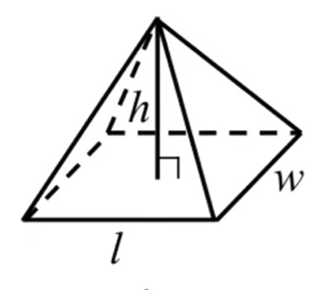
\includegraphics[width=0.55\linewidth]{images/cus51}
\end{center}
\begin{solution}
28
\end{solution}

\question[1]
At what value of $x$ will the expression $2\sqrt{x^4}$ be equivalent to $1152$?
\begin{solution}
$\pm 24$
\end{solution}



\newpage




\question[1]
If $80\%$ of a number is $104$, what is $40\%$ of the same number?
\begin{solution}
52
\end{solution}

\question[1]
When graphed in the $xy$-plane, line $m$ passes through the points $(-5, -4)$ and $(15, 4)$. If line $n$ is perpendicular to line $m$, which of the following could be the equation of line $n$?
\begin{choices}
  \CorrectChoice $y = -\frac{5}{2}x + 2$
  \choice $y = -\frac{5}{4}x - 3$
  \choice $y = \frac{2}{5}x + 6$
  \choice $y = \frac{5}{2}x + 10$
\end{choices}

\question[1]
The graph of the function $g(x)$ is shown. If $h(x)=g(x)+4$, what is the value of $h(6)$?
\begin{center}
  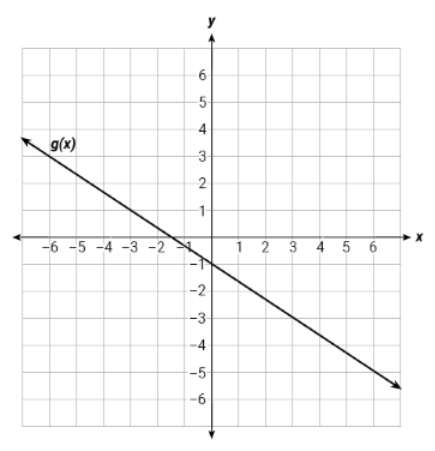
\includegraphics[width=0.75\linewidth]{images/cus41}
\end{center}
\begin{solutionorbox}
\end{solutionorbox}



\newpage




\question[1]
The function $h(t)=-4.9 t^2+14.7 t+19.6$ determines the height of a cannonball from the ground, in meters, $t$ seconds after it is fired from a cannon over a cliff. How long, in seconds, is the cannonball in the air before it touches the ground?
\begin{choices}
  \choice 1
  \CorrectChoice 4
  \choice 14.7
  \choice 19.6
\end{choices}



\question[1]
The function $p(t)$ gives the population of bees, in thousands, in a park over $t$ years since data was first collected in 2008. The function is graphed on the coordinate plane. Which statement is the best interpretation of where the graph intersects the $p(t)$ axis?
\begin{center}
  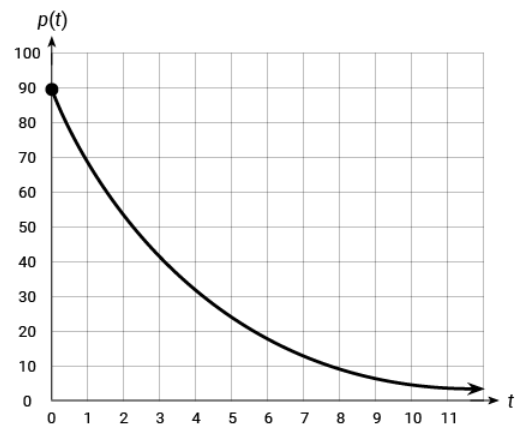
\includegraphics[width=0.75\linewidth]{images/cus42}
\end{center}
\begin{choices}
  \choice There were 90 bees in the park in 2008.
  \choice The total number of bees between 2008 and 2019 decreased by 90.
  \choice There were 90,000 bees in the park in 2008.
  \choice There were 90,000 bees in the park in 1997.
\end{choices}



\newpage




\question[1]
The circumference of a circle is equal to $w \pi$ feet, and the area of a circle is equal to $w \pi$ square feet, where $w$ is a constant. What is the value of $w$?
\begin{choices}
  \choice 1
  \choice 2
  \CorrectChoice 4
  \choice 8
\end{choices}

\question[1]
Line $m$ has an equation $A x+B y=C$. If line $m$ passes through the points $(0,6)$ and $(-15,0)$, what is the value of $-\frac{A}{B}$?
\begin{solution}
$\frac{2}{5}$
\end{solution}


\question[1]
Consider the quadratic equation:
\[
  3 x^2-6 x-11=0
\]
If one of the solutions to the given quadratic equation is $\frac{3+\sqrt{g}}{3}$, what is the value of $g$?
\begin{solution}
42
\end{solution}



\newpage




\question[1]
Consider the equation:
\[
  27 x^2+k x+12=0
\]
In the given equation, $k$ is a constant. For which of the following values of $k$ will the equation have no real solutions?
\begin{choices}
  \choice -55
  \choice -36
  \CorrectChoice 34
  \choice 40
\end{choices}

\question[1]
A high school gave a survey to all of its students. It was determined that $28\%$ of the students are ninth graders. Out of all the ninth graders, $15\%$ walk to school. If 21 ninth graders walk to school, how many students attend the high school in total?
\begin{solution}
500
\end{solution}

\question[1]
Consider the system of equations:
\[
  \begin{gathered}
  9 x-8 y=-26 \\
  5 x-6 y=-30
  \end{gathered}
\]
The coordinate point $(x, y)$ is the solution to the system of equations shown. What is the value of $x+y$?
\begin{choices}
  \choice 4
  \choice 6
  \choice 10
  \CorrectChoice 16
\end{choices}



\newpage




\question[1]
In the figure shown, what is the length of side $CD$, in centimeters?
\begin{center}
  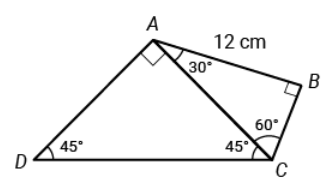
\includegraphics[width=0.75\linewidth]{images/cus43}
\end{center}
\begin{choices}
  \choice $4 \sqrt{6}$
  \choice $8 \sqrt{3}$
  \choice $6 \sqrt{6}$
  \choice $8 \sqrt{6}$
\end{choices}

\question[1]
Mr. Corbin recently had his students take a physics test. He made a mistake on one of the test questions, so Mr. Corbin added 10 points to every student's score. The histogram summarizes the test scores after adding the 10 extra points. In which range is the median score before the 10 points were added?
\begin{center}
  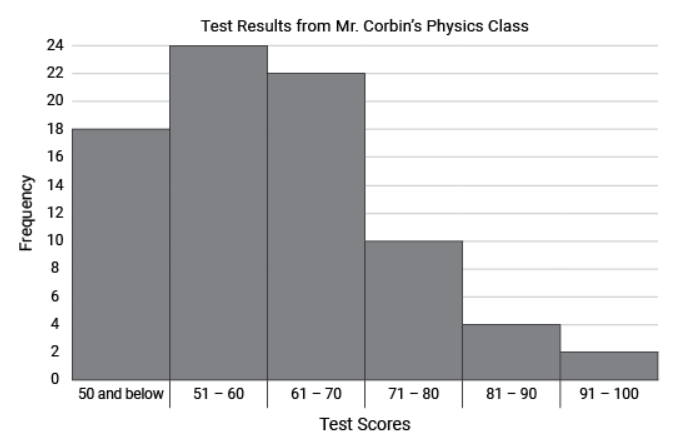
\includegraphics[width=0.75\linewidth]{images/cus44}
\end{center}
\begin{choices}
  \choice 50 and below
  \choice 51-60
  \choice 61-70
  \choice 71-80
\end{choices}



\newpage




\question[1]
In the $xy$-plane, the graph of $y=4 x^2-48 x+44$ intersects the line $y=b$ at exactly one point. What is the value of $b$?
\begin{choices}
  \CorrectChoice -100
  \choice -1
  \choice 6
  \choice 11
\end{choices}

\question[1]
What value of $x$ satisfies the given equation?
\[
  \frac{2 x^2}{x^2-4}+\frac{7 x}{x+2}=\frac{-2}{x-2}
\]
\begin{choices}
  \choice -2
  \choice $-\frac{2}{3}$
  \CorrectChoice $\frac{2}{3}$
  \choice 2
\end{choices}

\question[1]
A school budgets $\$1,600$ to buy pens. A bulk order of pens requires a minimum purchase of at least 520 pens for a discounted price. The store charges $\$2$ per black pen and $\$4$ per blue pen. What is the maximum number of blue pens the school can order to stay within budget and receive the discounted price?
\begin{solution}
280
\end{solution}



\newpage




\question[1]
Consider the expression:
\[
  0.84 y^2-7.2 y+1.56
\]
The given expression is equivalent to 
\[
  k\left(-7 y^2+60 y-13\right)
\]
, where $k$ is a constant. What is the value of $k$?
$k$ is a constant. What is the value of $k$?
\begin{solution}
$-\frac{3}{25}$
\end{solution}

\question[1]
Consider the equation:
\[
  b^{\frac{4}{5}}=c^{\frac{2}{3}}
\]
Given the equation above, if $c=b^{2 a+1}$, then what is the value of $a$?
\begin{solution}
$\frac{1}{10}$
\end{solution}

\question[1]
A ramen restaurant tracked how many orders they received during the first 6 hours of opening. The scatterplot shows the results. Which of the following equations best models the data in the scatterplot?
\begin{center}
  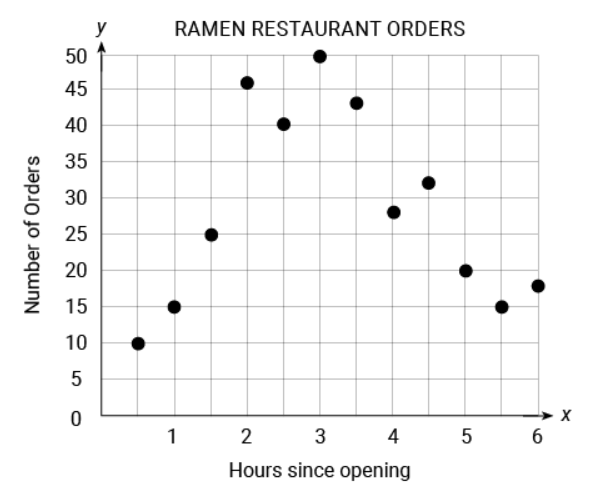
\includegraphics[width=0.75\linewidth]{images/cus45}
\end{center}
\begin{choices}
  \choice $y=-4.21 x^2+26.97 x-2.09$
  \choice $y=-4.21 x^2-26.97 x-2.09$
  \choice $y=4.21 x^2+26.97 x+2.09$
  \choice $y=4.21 x^2-26.97 x+2.09$
\end{choices}



\newpage




\question[1]
The center point of circle $Q$ when graphed in the $xy$-plane is $(4,6)$. The coordinate $(4,11)$ is on the circumference of the circle. What is the diameter of circle $Q$?
\begin{choices}
  \choice 4
  \choice 5
  \CorrectChoice 10
  \choice 12
\end{choices}

\question[1]
Consider the equation:
\[
  3 x-x(7-8)+12=4 x-(6 x+18)
\]
In the given equation, what is the value of $x$?
\begin{choices}
  \CorrectChoice -5
  \choice -1
  \choice 1
  \choice 5
\end{choices}

\question[1]
The equation for line $p$ is $5 x-8 y=40$. Line $q$ is perpendicular to line $p$ and passes through the point $(10,0)$. What is the equation for line $q$?
\begin{choices}
  \CorrectChoice $y=-\frac{8}{5} x+16$
  \choice $y=-\frac{8}{5} x+10$
  \choice $y=\frac{5}{8} x+16$
  \choice $y=\frac{5}{8} x+10$
\end{choices}



\newpage




\question[1]
The graph shows how much money $f(x)$ Maya saves over $x$ months. What is the best interpretation of the slope of the function $f(x)$?
\begin{center}
  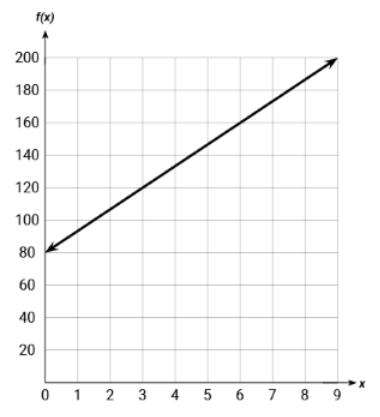
\includegraphics[width=0.75\linewidth]{images/cus46}
\end{center}
\begin{choices}
  \choice Maya saves $\$20$ each month.
  \choice Maya saves $\$40$ every 3 months.
  \choice Maya saves $\$80$ each month.
  \choice Maya saves $\$120$ in a year.
\end{choices}

\question[1]
Yuv is purchasing shoes that originally cost $\$200$. The store is having a $20\%$ off sale. Yuv has a coupon for an additional $10\%$ off that is applied after the store discount. He can determine the price of the shoes with both discounts by calculating $(200)(p)$. What is the value of $p$?
\begin{solution}
0.72
\end{solution}



\newpage




\question[1]
A number of racecar racers continuously go around a track. The scatterplot shows the distribution of how many laps the racers could complete after a certain time. If $y$ is the number of laps and $x$ is the time in hours, which of the following is a line that most closely fits the data?
\begin{center}
  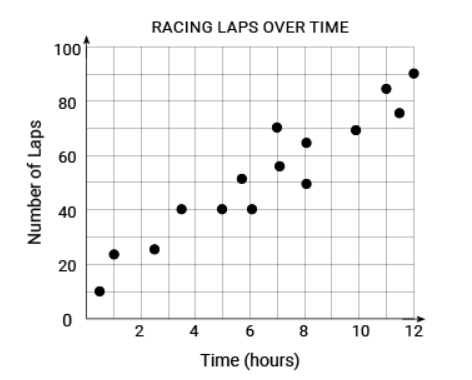
\includegraphics[width=0.75\linewidth]{images/cus47}
\end{center}
\begin{choices}
  \choice $y=0.7 x+15$
  \choice $y=2 x+30$
  \choice $y=7 x+10$
  \choice $y=10 x$
\end{choices}

\question[1]
The diagonal of a rectangle is 26 meters. The width of the rectangle is 10 meters. What is the area of the rectangle, in square meters?
\begin{choices}
  \choice 120
  \choice 130
  \CorrectChoice 240
  \choice 260
\end{choices}



\newpage




\question[1]
Martha wants to know what dances are popular on social media platforms she uses by conducting a survey. Which group of people should Martha survey to get the most accurate data?
\begin{choices}
  \choice A random sample of followers on a random social media platform
  \CorrectChoice A random sample of users of all the social media platforms that Martha uses
  \choice A random sample of users who follow Martha across all of her social media platforms
  \choice A random sample of Martha's followers who are also dancers
\end{choices}

\question[1]
What values of $x$ satisfy the given equation?
\[
  x^2-6 x+7=0
\]
\begin{choices}
  \choice $x=1$ and $x=7$
  \choice $x=-1$ and $x=-7$
  \CorrectChoice $x=3+\sqrt{2}$ and $x=3-\sqrt{2}$
  \choice $x=-3+\sqrt{2}$ and $x=-3-\sqrt{2}$
\end{choices}

\question[1]
Consider the expression:
\[
  \frac{3 x+2}{a x+5}+2 x-3=\frac{8 x^2+x-13}{a x+5}
\]
In the expression above, $x \neq \frac{-5}{a}$ and $a$ is a non-zero constant. What is the value of $a$?
\begin{choices}
  \choice -4
  \choice $-\frac{1}{3}$
  \choice 2
  \CorrectChoice 4
\end{choices}

\endgradingrange{sat-drill-13}
